\documentclass[12pt,letterpaper]{article}
\usepackage[utf8]{inputenc}
\usepackage{amsmath,amssymb,amsthm}
\usepackage{graphicx}
\usepackage{natbib}
\usepackage{booktabs}
\usepackage{setspace}
\usepackage{geometry}
\usepackage[colorlinks=true,citecolor=blue,linkcolor=blue]{hyperref}
\geometry{margin=1.1in}

\newtheorem{theorem}{Theorem}
\newtheorem{proposition}{Proposition}
\newtheorem{lemma}{Lemma}
\newtheorem{corollary}{Corollary}
\newtheorem{assumption}{Assumption}
\newtheorem{remark}{Remark}
\theoremstyle{definition}
\newtheorem{definition}{Definition}

\newcommand{\Lists}{\mathbf{Lists}}
\newcommand{\R}{\mathbb{R}}
\newcommand{\md}[1]{\textcolor{red}{[#1]}} % margin note command for coauthor comments
\usepackage{xcolor}

\title{The Market for Elite Status\thanks{Working draft --- not for circulation.
Derivations in the appendices are machine-verified; see \texttt{analysis/static\_model.py}
in the project repository.}}
\author{Jo\~{a}o Ricardo Faria\\ Florida Atlantic University
  \and Michael D. Ryall\\ Florida Atlantic University}
\date{\today}

\begin{document}

\maketitle

\begin{abstract}
\noindent Why does competition not eliminate elite institutions that consume more
resources than they produce? We model a market for elite status in the general
equilibrium clubs framework of Ellickson, Grodal, Scotchmer, and Zame: elite schools
sell memberships that confer status but no skill; elite-managed firms are strictly less
productive than their competently managed rivals; all memberships are competitively
priced. We show that strictly less productive elite firms operate in equilibrium
whenever the status discount accepted by elite managers exceeds the compensating
differential demanded by their employees plus the resources burned in status
production. Aggregate output falls monotonically as the taste for status spreads ---
indeed it falls even when elite firms are more productive per unit of output, provided
they are less productive per unit of resources. Yet every such equilibrium lies in the
core and is Pareto optimal: no entrant, coalition, or policy commanding lump-sum
instruments can profitably displace the elite sector. Markets work; material
efficiency does not follow. The welfare theorem fails only when status is
\emph{positional} --- valued for its scarcity. Then the equilibrium remains unique
but exhibits over-entry into elite institutions: each entrant dilutes the status of
every incumbent, an economy-wide externality that membership prices cannot register.
Equilibria are no longer in the core, and a tax on elite memberships raises both
welfare and output. [Abstract to be finalized with the dynamic section.]
\end{abstract}

\onehalfspacing

\section{Introduction}\label{sec:intro}

\emph{[Working draft of the introduction. To be finalized last, per the project plan.]}

A familiar argument holds that competitive markets discipline waste: an institution
that consumes more resources than it returns should be undercut by rivals and
disappear. Elite institutions appear to defy this logic. Elite universities charge
extraordinary tuition while their measurable value-added is contested; the firms that
preferentially hire their graduates pay premia that are difficult to attribute to
productivity; and both have persisted, and indeed expanded, over decades of intense
competition in product, labor, and education markets.

This paper's answer is not that competition fails, but that it succeeds. We model
elite status as what it observably is: a membership --- in a school, and subsequently
in the class of people who run certain firms --- that is bought and sold at market
prices. The natural home for such a model is the general equilibrium theory of clubs
developed by \citet{ellickson1999clubs,ellickson2001clubs,ellickson2006organization},
in which group memberships are priced alongside ordinary commodities and agents care
about the characteristics of their fellow members. Within that framework we obtain
three results.

First, strictly less productive elite-managed firms operate in competitive equilibrium
under a transparent condition: the pay cut that status-seeking managers accept must
cover the compensating differential demanded by the workers they manage plus the
resources burned by elite institutions in producing status
(Proposition~\ref{prop:coexist}). The waste is financed by identified parties at
market prices; no friction, information asymmetry, or market power is involved.

Second, as the taste for status spreads through the population, aggregate output falls
monotonically (Proposition~\ref{prop:decline}). The condition for decline is weaker
than elite firms being less productive: output falls whenever the elite sector
produces less output \emph{per unit of resources consumed}, which can hold even when
elite firms produce more output per firm.

Third --- and centrally --- every such equilibrium lies in the core of the economy and
is Pareto optimal (Theorem~\ref{thm:nocorrection}). No entrant offering ``status
without waste,'' no coalition of workers and investors, and no policymaker restricted
to lump-sum instruments can achieve a Pareto improvement. The market has nothing to
correct: falling measured output is the equilibrium price of status consumption. The
popular syllogism ``markets work, therefore materially wasteful institutions cannot
survive competition'' commits a non sequitur, and the point of this paper is to locate
it precisely. Markets work; material efficiency does not follow.

The efficiency of the baseline is not a celebration; it is a diagnosis. It locates
exactly where a genuine market failure must live if there is one: not in the waste,
which is priced, but in the \emph{relativity} of status. Section~\ref{sec:positional}
makes status positional --- valuable because others lack it --- so that each entrant
into the elite dilutes the status of every incumbent. This economy-wide externality
lies outside the assumptions of the clubs welfare theorems: membership prices
internalize composition effects \emph{within} a group, but eliteness is a
characteristic of a class that spans all elite groups. The positional equilibrium
exists, is unique, and self-limits (dilution shrinks the elite), but it is no longer
Pareto optimal and no longer in the core (Propositions~\ref{prop:positional}
and~\ref{prop:inefficiency}): there is over-entry into elite institutions, and a
Pigouvian tax on elite memberships raises welfare \emph{and} output
(Proposition~\ref{prop:tax}). The contrast between Theorem~\ref{thm:nocorrection}
and Proposition~\ref{prop:inefficiency} is the paper's answer to when elite waste is
and is not a policy problem: absolute status is efficient consumption; positional
status is a rat race.

\emph{[Planned: a paragraph previewing the overlapping-generations dynamics, in
which the spread of status preferences interacts with wealth accumulation.]}

\section{Related Literature}\label{sec:lit}

\emph{[Skeleton --- each paragraph states the confrontation to be developed.]}

\textbf{Markets for status.} \citet{beckermurphywerning2005} price status as a
divisible good in fixed supply traded in a hedonic market. We differ in making the
supply side explicit: status here is membership in clubs --- schools and firms ---
produced by institutions with real resource costs, priced by the membership prices of
\citet{ellickson1999clubs}, with a production economy attached. \citet{colemailathpostlewaite1992}
generate status-driven distortions from matching norms; our status is marketed, not
normed, which yields prices, entry margins, and comparative statics that norms models
do not deliver. \citet{moldovanuselashi2007}, \citet{board2009group}, and
\citet{rayo2013signal} study a single designer selling status categories or exclusivity;
here the supply of status is competitive and embedded in general equilibrium.

\textbf{Status and allocation.} \citet{fershtmanmurphyweiss1996} show occupational
status concerns distort the allocation of talent in growth. Our persistence result is
at the level of the \emph{firm}: identifiable, less productive organizations survive
because their control rights are bundled with status consumption. The rat-race
tradition (\citealt{akerlof1976caste}; \citealt{hopkinskornienko2004};
\citealt{frank1985demand}; \citealt{hirsch1976social}) delivers genuine inefficiency
from relative comparison; in our baseline there is no externality and hence no rat
race --- that distinction is the point of Theorem~\ref{thm:nocorrection}, and
Section~\ref{sec:positional} shows exactly what must be added to overturn it,
using the widespread-externalities equilibrium concept of
\citet{noguchizame2006externalities}.
\citet{kimtertiltyum2024} provide a recent quantitative treatment of education-status
externalities; we provide the institutional theory.

\textbf{Education and elite institutions.} In \citet{spence1973signaling} education is
informative about hidden types; our elite school conveys no information --- there are
no hidden types --- and its product is the membership itself. This places us closest
to the reputation-and-selection view of schooling of \citet{macleodurquiola2019} and
to the evidence that elite institutions' value operates through access and affiliation
rather than skill production (\citealt{zimmerman2019elite};
\citealt{michelmanpricezimmerman2022}; \citealt{chettydemingfriedman2026};
\citealt{dalekrueger2002}; \citealt{rivera2015pedigree}). We treat the zero-teaching
elite school as a polar case; \citet{arteaga2018} shows content matters even at elite
institutions, and nothing in our results requires the polar case
(Remark~\ref{rem:polar}). Prior applied uses of the clubs machinery are rare; the
main exceptions are \citet{caucutt2001peer,caucutt2002vouchers} on schooling with
peer effects, and the firms-as-clubs analyses of \citet{prescotttownsend2006firms}
and \citet{zame2007incentives}.

\textbf{Dynamics (planned).} The dynamic section will engage
\citet{murphyshleifervishny1991}, \citet{baumol1990entrepreneurship},
\citet{acemoglu1995reward}, \citet{hasslermora2000}, \citet{galorzeira1993},
\citet{durlauf1996persistent}, and \citet{doepkezilibotti2008} --- in particular,
explaining why the selection dynamic that eliminates unproductive aristocracies in
\citet{doepkezilibotti2008} is blocked when status is competitively priced.

\section{The Framework}\label{sec:framework}

We adopt the general equilibrium model of groups of
\citet{ellickson2006organization}, which extends \citet{ellickson1999clubs} to allow
groups to produce outputs and memberships to carry acquired characteristics. We state
the primitives compactly and refer the reader to the source for full detail.

\subsection{Commodities, groups, and memberships}

There are $N$ divisible, publicly traded private goods. Groups are described by a
finite set $\mathcal{G}$ of \emph{group types} $(\pi,\gamma,y)$: a \emph{profile}
$\pi:\Omega\rightarrow\mathbb{Z}_+$ specifying how many members with each
\emph{membership characteristic} $\omega\in\Omega$ the group requires; an
\emph{organizational characteristic} $\gamma\in\Gamma$; and an \emph{input--output
vector} $y\in\R^N$, with negative components inputs and positive components outputs.
A \emph{membership} is a pair $m=(\omega,(\pi,\gamma,y))$ with $\pi(\omega)\geq 1$;
$\mathcal{M}$ denotes the (finite) set of memberships. A \emph{list} is a function
$\ell:\mathcal{M}\rightarrow\mathbb{Z}_+$; $\Lists$ denotes the set of lists.

\subsection{Agents}

The set of agents is a nonatomic finite measure space $(A,\mathcal{F},\lambda)$. An
agent $a$ is described by a consumption set $X_a\subset\R^N_+\times\Lists$ (closed,
allowing free disposal upward in private goods, with a uniform bound on list sizes),
an endowment $(e_a,0)\in X_a$ of private goods and no memberships, and a utility
function $u_a:X_a\rightarrow\R$, continuous and strictly increasing in private goods
for each fixed list. Consumption sets encode qualification requirements: a choice
$(x_a,\ell_a)$ is feasible only if $a$ can fulfill the requirements of every
membership in $\ell_a$, and characteristics may be \emph{acquired} by holding other
memberships (e.g., a degree qualifies its holder for a managerial role). The economy
is the measurable mapping $a\mapsto(X_a,e_a,u_a)$.

\subsection{States and equilibrium}

A \emph{state} $(x,\mu):A\rightarrow\R^N\times\R^{\mathcal{M}}$ assigns private goods
and lists. A state is \emph{feasible} if it is individually feasible, satisfies
material balance (aggregate consumption does not exceed aggregate endowment plus the
net output of the groups formed), and is \emph{consistent}: for every group type, the
aggregate choices of its various memberships are in the proportions $\pi$ requires, so
that agents can be matched into groups with no seat empty and no agent unmatched.

Prices are $(p,q)\in\R^N_+\times\R^{\mathcal{M}}$: $p$ for private goods, $q$ for
memberships. Membership prices may be positive (tuition), negative (wages), or zero.
A \emph{group equilibrium} is a price system $(p,q)$ with $p\neq 0$ and a feasible
state $(x,\mu)$ such that:
\begin{enumerate}
  \item \textbf{Budget balance for group types:} for each $(\pi,\gamma,y)\in\mathcal{G}$,
  $\sum_{\omega\in\Omega}\pi(\omega)\,q(\omega,(\pi,\gamma,y)) + p\cdot y = 0$.
  \item \textbf{Budget feasibility:} for almost all $a$,
  $(p,q)\cdot(x_a,\mu_a)\leq p\cdot e_a$.
  \item \textbf{Optimization:} for almost all $a$, any choice strictly preferred to
  $(x_a,\mu_a)$ costs strictly more than $p\cdot e_a$.
\end{enumerate}

Two results from \citet{ellickson2006organization} are used below. Their Theorem~1:
\emph{every group equilibrium state belongs to the core, and in particular is Pareto
optimal; if endowments are desirable, it belongs to the strong core and is strongly
Pareto optimal.} Their Theorem~2 provides existence under group irreducibility,
desirable endowments, and uniformly bounded endowments; our analysis will not need it,
because we exhibit equilibria in closed form.

\section{An Economy with a Market for Elite Status}\label{sec:model}

\subsection{Goods, group types, and memberships}

There are two private goods: an input good $y_1$ (``resources,'' the num\'{e}raire)
and a consumption good $y_2$ with price $p_2$. Membership characteristics are
$\Omega=\{S, M, EM, L\}$: student, manager, elite manager, laborer. There are four
group types:
\begin{align*}
  g_1 &= \big((S);\, s;\, (-r,0)\big)
    && \text{serious school: educates one student at resource cost } r>0,\\
  g_2 &= \big((S);\, s^\ast;\, (-\tau r,0)\big)
    && \text{elite school: } \tau\geq 1,\\
  g_3 &= \big((M,2L);\, f;\, (-c,\phi)\big)
    && \text{competent firm: one manager, two laborers},\\
  g_4 &= \big((EM,2L);\, f^\ast;\, (-\beta c,\alpha\phi)\big)
    && \text{elite firm: } \beta\geq 1,\ \alpha>0.
\end{align*}
The parameter $\tau$ measures the resources elite schools devote to the production of
status rather than skill; $\beta$ measures the excess resource use of elite-managed
firms; $\alpha$ their output multiplier. The interesting configuration, though not
the only one we analyze, is $\tau>1$, $\beta>1$, $\alpha\leq 1$: elite institutions
burn resources, and elite firms produce no more than competent ones.

The memberships are $m_1=(S,g_1)$, $m_2=(S,g_2)$, $m_{3.1}=(M,g_3)$,
$m_{3.2}=(L,g_3)$, $m_{4.1}=(EM,g_4)$, $m_{4.2}=(L,g_4)$.

\subsection{Agents}

Agents form a continuum of measure one. Each is endowed with $e=(k,0)$, $k>0$.
Agents may attend at most one school and hold at most one job. The characteristic
$M$ is acquired at a serious school and $EM$ at an elite school:\ a choice with
$\ell(m_{3.1})\geq 1$ is feasible only if $\ell(m_1)\geq 1$, and $\ell(m_{4.1})\geq 1$
only if $\ell(m_2)\geq 1$. The characteristic $L$ requires no schooling.

Agents differ in a single taste parameter $\eta\geq 0$, distributed according to an
atomless distribution function $F$, strictly increasing on its support $[0,\bar\eta)$
with $\bar\eta\leq\infty$. Preferences are
\begin{equation}\label{eq:utility}
  u(x,\ell;\eta) \;=\; D(\ell;\eta)\, h(x_1,x_2),
  \qquad h(x_1,x_2)=\sqrt{x_1 x_2},
\end{equation}
where $D$ is built multiplicatively from the list:\ attending any school contributes a
factor $\delta_s\in(0,1)$; working as a manager a factor $\delta_m\in(0,1)$; working
as a laborer a factor $\delta_l\in(0,1)$; holding the elite-manager membership
$m_{4.1}$ contributes the additional factor $(1+\eta)$ --- this is the utility of
elite status --- and holding the elite-firm laborer membership $m_{4.2}$ the factor
$(1-\chi)$, $\chi\in[0,1)$, reflecting distaste for working under elite management.
Thus, for the five undominated vocational choices,
\[
D = \begin{cases}
  1 & \text{leisure (empty list)},\\
  \delta_s\delta_m(1+\eta) & \text{elite manager } (\ell(m_2)=\ell(m_{4.1})=1),\\
  \delta_s\delta_m & \text{competent manager } (\ell(m_1)=\ell(m_{3.1})=1),\\
  \delta_l & \text{laborer, competent firm } (\ell(m_{3.2})=1),\\
  \delta_l(1-\chi) & \text{laborer, elite firm } (\ell(m_{4.2})=1).
\end{cases}
\]
All other feasible lists (school without subsequent employment, schooling combined
with labor, double schooling) are strictly dominated at any prices arising in
equilibrium; Lemma~\ref{lem:dominated} in Appendix~\ref{app:derivations} verifies
this. Note that status attaches to the \emph{elite-manager membership}: the elite
school is the gate, not the prize.

It is convenient to write
\[
\mu \equiv \frac{1}{\delta_s\delta_m}>1, \qquad
\lambda \equiv \frac{1}{\delta_l}>1, \qquad
\lambda^{e} \equiv \frac{\lambda}{1-\chi}\geq\lambda .
\]

\begin{remark}\label{rem:polar}
The elite school teaches nothing and the elite firm wastes resources by assumption;
these are polar cases chosen for transparency, not necessity. All results below
depend only on the composite parameters $(\tau,\beta,\alpha)$, so a reader who
prefers elite schools that teach something (but less per dollar) may set $\tau$
accordingly without change to the analysis.
\end{remark}

\section{Equilibrium}\label{sec:equilibrium}

Because $h$ is homothetic, an agent with net income $w$ (endowment value net of
membership prices) demands $x_1=w/2$, $x_2=w/(2p_2)$ and attains indirect utility
$D\, w/(2\sqrt{p_2})$. All occupational comparisons are therefore rankings of
$D\cdot w$, independent of $p_2$.

\subsection{Characterization}

Occupational indifference for the (atomless) population pins down net incomes. Since
leisure yields $D\cdot w = k$, participation of laborers and competent managers
requires
\begin{equation}\label{eq:wages}
  w_M = \mu k, \qquad w_L = \lambda k, \qquad w_{L^\ast} = \lambda^{e} k,
\end{equation}
and the elite-manager income satisfies, for a \emph{marginal} type $\eta^\ast$,
\begin{equation}\label{eq:cutoff}
  w_E = \frac{\mu k}{1+\eta^\ast},
\end{equation}
with all types $\eta>\eta^\ast$ strictly preferring the elite path and all
$\eta<\eta^\ast$ strictly avoiding it. Membership prices follow from the definition
of net income ($w = k - \text{fees} + \text{wages}$) and budget balance of the
schools:
\begin{equation}\label{eq:prices}
  q_1 = r,\quad q_2=\tau r,\quad
  q_{3.1} = k - r - \mu k,\quad
  q_{3.2} = k - \lambda k,\quad
  q_{4.1} = k - \tau r - w_E,\quad
  q_{4.2} = k - \lambda^{e} k .
\end{equation}
Budget balance for competent firms determines the output price,
\begin{equation}\label{eq:p2}
  p_2\phi = c + r + (\mu + 2\lambda - 3)k \;>\;0,
\end{equation}
and budget balance for elite firms determines the cutoff. Define
\begin{equation}\label{eq:Z}
  Z \;\equiv\; \alpha\big[c + r + (\mu+2\lambda-3)k\big] \;-\; \beta c \;-\; \tau r
  \;+\; (3 - 2\lambda^{e})k .
\end{equation}
Then the elite-firm budget balances if and only if $w_E = Z$, i.e.,
\begin{equation}\label{eq:etastar}
  1+\eta^\ast \;=\; \frac{\mu k}{Z}.
\end{equation}
The measure of elite managers is $m^\ast = 1-F(\eta^\ast)$; consistency requires the
elite sector to employ $2m^\ast$ laborers and the competent sector, of measure $n$
firms, to employ $n$ managers and $2n$ laborers. Market clearing in the input good,
\begin{equation}\label{eq:clearing}
  \underbrace{\sigma_0\frac{k}{2}
  + m^\ast\frac{w_E}{2} + 2m^\ast\frac{w_{L^\ast}}{2}
  + n\frac{w_M}{2} + 2n\frac{w_L}{2}}_{\text{consumption demand}}
  + \underbrace{m^\ast(\tau r + \beta c) + n(r+c)}_{\text{resource use}}
  \;=\; k,
\end{equation}
with $\sigma_0 = 1 - 3m^\ast - 3n$ the leisure share, determines $n$ linearly;
clearing of the consumption good follows by Walras' law
(Appendix~\ref{app:derivations}).

\begin{assumption}[Interior configuration]\label{ass:interior}
Parameters are such that (i) $0 < Z < \mu k$; (ii) $F(\eta^\ast)<1$; (iii) the
solution $n$ of \eqref{eq:clearing} is strictly positive; and (iv) $\sigma_0\geq 0$.
\end{assumption}

Part (i) puts the cutoff in the interior: if $Z\leq 0$, elite firms cannot break even
even with unpaid managers and the elite sector is empty; if $Z\geq\mu k$, every agent
joins it. Parts (ii)--(iv) ensure all sectors coexist. The parameterization of
Section~\ref{sec:example} satisfies all four.

\begin{lemma}\label{lem:characterization}
Under Assumption~\ref{ass:interior}, the prices
\eqref{eq:prices}--\eqref{eq:p2} and the state in which agents with
$\eta>\eta^\ast$ sort into elite management, measures $n$, $2n$, and $2m^\ast$ of
agents with $\eta<\eta^\ast$ sort into competent management, competent labor, and
elite labor respectively, and the remainder choose leisure, constitute a group
equilibrium. Every group equilibrium in which all six memberships are chosen by a
positive measure of agents has these prices, and its cutoff, sector sizes, and
allocation are given by \eqref{eq:cutoff}--\eqref{eq:clearing}.
\end{lemma}

The proof (Appendix~\ref{app:derivations}) verifies budget balance, budget
feasibility, consistency, and --- using Lemma~\ref{lem:dominated} --- optimization
over every feasible list.

Two features deserve notice. First, elite managers \emph{accept a status discount}:
$w_E<w_M$, with the discount $\mu k\,\eta^\ast/(1+\eta^\ast)$ increasing in the
equilibrium cutoff. In membership-price terms, $q_{4.1}>q_{3.1}$: the elite-manager
seat is the more expensive to occupy. Second, laborers in elite firms are paid a
compensating differential, $w_{L^\ast}>w_L$: as
\citet[p.~151]{ellickson2006organization} anticipate, firms offering uncongenial
conditions must pay more.

\subsection{When do wasteful elite firms survive?}

\begin{proposition}[Coexistence]\label{prop:coexist}
Under Assumption~\ref{ass:interior}, an equilibrium with an active elite sector of
strictly lower output productivity ($\alpha<1$) exists if and only if, at the
equilibrium cutoff $\eta^\ast$,
\begin{equation}\label{eq:coexist}
  \underbrace{(w_M - w_E)}_{\text{status discount}}
  \;>\;
  \underbrace{2\,(w_{L^\ast} - w_L)}_{\text{compensating differential}}
  \;+\;
  \underbrace{(\beta-1)c + (\tau-1)r}_{\text{resources burned}} .
\end{equation}
\end{proposition}

The economics is an accounting identity made competitive: the elite firm's revenue
shortfall relative to a competent firm must be financed within the group, and the only
willing financier is the manager who values the membership itself. The status
discount conceded by the marginal elite manager must cover both the premium demanded
by the two laborers who would rather work elsewhere and the resources burned by the
elite school and the elite firm's own inefficiency. No cross-subsidy from outside the
group is possible --- budget balance for group types forbids it --- so the entire
institution of wasteful eliteness is self-financing, at market prices, out of the
demand for status.

\subsection{The spread of status preferences and the decline of output}

Aggregate output of the consumption good is $Y=\phi\,(n+\alpha m^\ast)$. Consider a
first-order stochastically dominating shift of the taste distribution $F$ --- more
people care more about status. By \eqref{eq:etastar} the cutoff $\eta^\ast$ depends
only on prices and technology, \emph{not} on $F$; hence the elite sector expands
mechanically, $m^\ast = 1-F(\eta^\ast)$ rising with the shift.

\begin{proposition}[Efficient decline]\label{prop:decline}
Under Assumption~\ref{ass:interior}, a FOSD shift of $F$ strictly increases the mass
of elite managers and firms and strictly decreases aggregate output if and only if
\begin{equation}\label{eq:decline}
  \frac{\alpha\phi}{\beta c + \tau r} \;<\; \frac{\phi}{c+r},
\end{equation}
i.e., if and only if the elite sector produces less output per unit of resources than
the competent sector. In particular, output declines whenever $\alpha\leq 1$ and
$(\tau-1)r+(\beta-1)c>0$; but it also declines for a range of $\alpha>1$.
\end{proposition}

Condition \eqref{eq:decline} is strictly weaker than $\alpha<1$: an elite sector
whose firms produce \emph{more} output than competent firms still drags aggregate
output down if its schools and firms consume disproportionately more resources.
Measured productivity statistics will register this as declining aggregate TFP.

\subsection{The market cannot correct it}

\begin{theorem}[No market correction]\label{thm:nocorrection}
Every equilibrium of Lemma~\ref{lem:characterization} belongs to the core of the
economy and is strongly Pareto optimal. Consequently: (i) no feasible reallocation
--- including any that shuts the elite sector, redirects its resources, or introduces
any group type in $\mathcal{G}$ in any proportion --- makes almost all agents better
off without making a positive measure worse off; (ii) no coalition of agents, of any
size, can profitably secede with any configuration of schools and firms; (iii) the
conclusion is unchanged as the taste for status spreads and output falls per
Proposition~\ref{prop:decline}.
\end{theorem}

\begin{proof}
The state is a group equilibrium (Lemma~\ref{lem:characterization}), so membership in
the core and Pareto optimality follow from Theorem~1 of
\citet{ellickson2006organization}. Strong Pareto optimality follows from the same
theorem once endowments are verified to be desirable, which is done in
Appendix~\ref{app:assumptions}.
\end{proof}

Theorem~\ref{thm:nocorrection} is the paper's central claim, and it is worth stating
what it does and does not say. It does not say the elite sector is harmless: output
falls, resources are burned, and the burn is real. It says the situation is not a
market failure. The waste is voluntarily financed by the people who consume the
status it produces, at prices that fully internalize its cost within each group.
Competition has no lever: an entrant offering ``elite status without the waste''
would have to offer the elite-manager membership at its equilibrium price, and the
equilibrium already prices every potential group type in $\mathcal{G}$. The familiar
inference --- markets discipline waste, elite waste persists, therefore markets must
be impeded --- fails at its first step. Markets discipline \emph{unpriced} waste.
Status is priced.

Three caveats delimit the result. First, the feasible set takes the group-type list
$\mathcal{G}$ as given; whether a status-conferring group type without resource burn
could exist is a question about what makes status credible.
Section~\ref{sec:positional} answers it: when status derives from scarcity, entry
self-dilutes, and exclusivity needs no artificial protection. Second, if status is
valued \emph{because others lack it}, utility depends on the economy-wide pattern of
memberships --- an externality outside the present framework, under which the
welfare theorem genuinely fails; that is the subject of
Section~\ref{sec:positional}. Third, welfare here is welfarist: status utility
counts. Section~\ref{sec:discussion} returns to this.

\section{Numerical Example}\label{sec:example}

Let $k=2$, $r=c=1$, $\tau=2$, $\beta=1.25$, $\alpha=0.9$, $\phi=6$,
$\delta_s=\delta_m=\tfrac12$ (so $\mu=4$), $\delta_l=\tfrac12$ (so $\lambda=2$),
$\chi=0.2$ (so $\lambda^{e}=2.5$), and let $\eta$ be exponentially distributed with
mean $s=0.3$. Elite schools cost twice what serious schools cost; elite firms use
25\% more input and produce 10\% less output.

Then $p_2=2$, $Z=3.55$, $\eta^\ast=89/71\approx 1.254$, and:
\begin{center}
\begin{tabular}{lcccc}
\toprule
 & elite manager & competent manager & laborer (elite firm) & laborer (comp.\ firm)\\
\midrule
net income $w$ & $3.55$ & $8$ & $5$ & $4$\\
membership price $q$ & $-3.55$ & $-7$ & $-3$ & $-2$\\
tuition paid & $2$ & $1$ & --- & ---\\
\bottomrule
\end{tabular}
\end{center}
The elite sector employs $3m^\ast\approx 4.6\%$ of the population
($m^\ast\approx 0.0153$), the competent sector $3n\approx 38.2\%$
($n\approx 0.1275$), and $\sigma_0\approx 57.2\%$ take leisure. Aggregate output is
$Y\approx 0.848$ and the resources burned are $m^\ast[(\beta-1)c+(\tau-1)r]\approx
0.019$. Condition \eqref{eq:coexist} holds: the status discount $8-3.55=4.45$
exceeds the compensating differential $2\times(5-4)=2$ plus the burn
$0.25+1=1.25$. Condition \eqref{eq:decline} holds as well
($\alpha(c+r)=1.8<\beta c+\tau r=3.25$).

Figure~\ref{fig:comparative} traces the equilibrium as the mean $s$ of the taste
distribution rises --- a FOSD shift. The elite sector expands, the competent sector
contracts, and output falls monotonically, while by Theorem~\ref{thm:nocorrection}
every point on the path is in the core.

\begin{figure}[t]
  \centering
  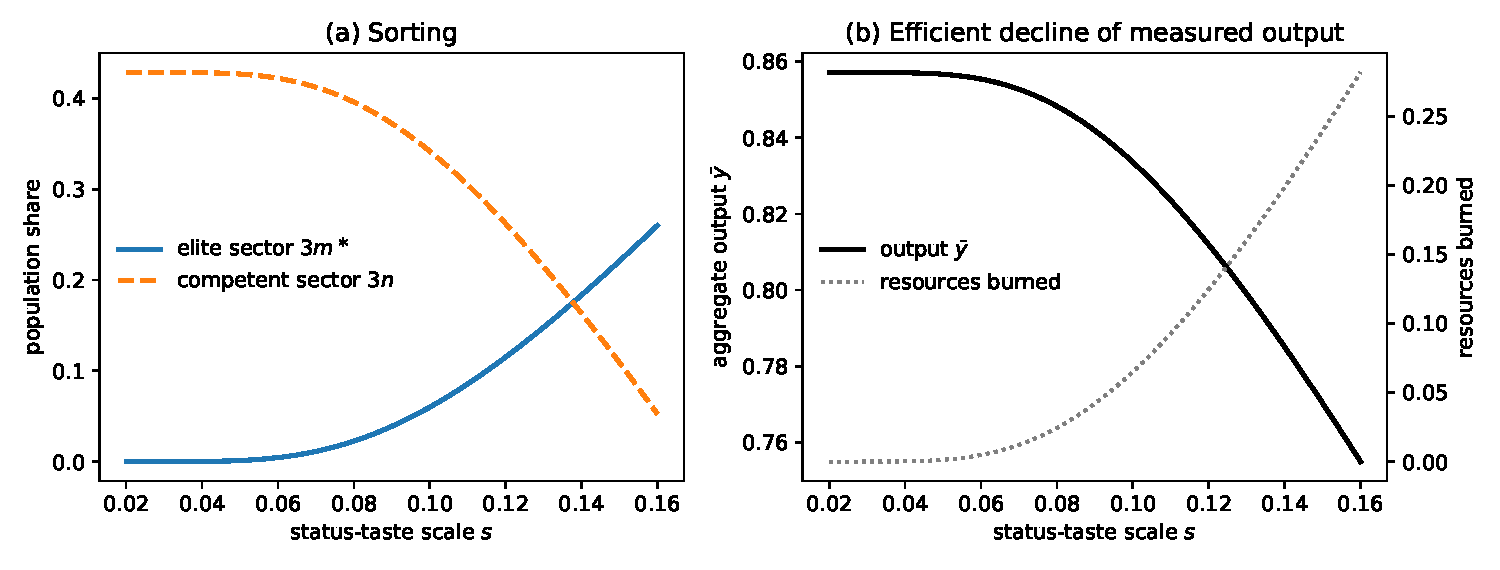
\includegraphics[width=\textwidth]{figures/status_taste_comparative_statics.pdf}
  \caption{Comparative statics in the status-taste scale $s$ ($\eta\sim$
  Exponential, mean $s$). Panel (a): population shares of the elite and competent
  sectors. Panel (b): aggregate output falls and burned resources rise as status
  taste spreads; every equilibrium shown is Pareto optimal
  (Theorem~\ref{thm:nocorrection}). Parameters as in Section~\ref{sec:example}.}
  \label{fig:comparative}
\end{figure}

\section{Positional Status and the Failure of the Welfare Theorem}\label{sec:positional}

Theorem~\ref{thm:nocorrection} rests on status being an \emph{absolute} amenity:
the elite-manager membership yields utility $(1+\eta)$ regardless of how many others
hold it. But much of what makes status status is scarcity
\citep{hirsch1976social,frank1985demand}: a credential everyone holds confers
distinction on no one. This section makes status positional and shows that
everything in Theorem~\ref{thm:nocorrection} breaks --- selectively, and in an
instructive way.

\subsection{Positional preferences and equilibrium}

Let $M$ denote the aggregate measure of agents holding the elite-manager membership
$m_{4.1}$, and replace the status factor $(1+\eta)$ in the utility specification of
Section~\ref{sec:model} with
\begin{equation}\label{eq:positional-utility}
  1 + \eta\, v(M),
\end{equation}
where $v:[0,1]\rightarrow(0,1]$ is continuous, strictly decreasing, with $v(0)=1$:
the value of eliteness falls as eliteness spreads. Each agent is negligible and
takes $M$ as given. Because utility now depends on \emph{other agents'}
memberships, preferences violate the assumptions of
\citet{ellickson2006organization}: this is a widespread externality in the sense of
\citet{noguchizame2006externalities}. We accordingly define a \emph{positional
group equilibrium} as prices $(p,q)$ and a feasible state $(x,\mu)$ satisfying the
three conditions of Section~\ref{sec:framework}, where optimization is with respect
to preferences \eqref{eq:positional-utility} evaluated at the aggregate elite mass
$M$ induced by the state itself.

Crucially, the externality operates at the level of the \emph{class} of elites ---
the holders of $m_{4.1}$ across all elite firms --- not at the level of any single
group. Membership prices internalize composition effects within a group; they have
no instrument that spans groups. This is precisely the gap in the price system that
the welfare theorem needs closed, and it is why the failure below is not a defect of
the clubs framework but a discovery made visible by it.

\subsection{Existence, uniqueness, and self-limiting eliteness}

The wages \eqref{eq:wages}, the output price \eqref{eq:p2}, and the elite-firm
break-even income $w_E=Z$ are untouched by the externality. The cutoff condition
becomes $(1+\eta^\ast v(M))\,\delta_s\delta_m\, w_E = k$, i.e.,
\begin{equation}\label{eq:positional-cutoff}
  \eta^\ast(M) \;=\; \frac{\eta^\ast_0}{v(M)},
\end{equation}
where $\eta^\ast_0 = \mu k/Z - 1$ is the cutoff of Section~\ref{sec:equilibrium}.
Consistency of the conjectured mass with sorting requires $M$ to be a fixed point of
\begin{equation}\label{eq:fixedpoint}
  \Phi(M) \;\equiv\; 1 - F\!\left(\frac{\eta^\ast_0}{v(M)}\right).
\end{equation}

\begin{proposition}[Positional equilibrium]\label{prop:positional}
Under Assumption~\ref{ass:interior} (applied at $M=M^\ast$), a positional group
equilibrium exists and its elite mass is unique: $\Phi$ is continuous and strictly
decreasing on $[0,1]$, so it has exactly one fixed point $M^\ast$. Moreover:
(i) $M^\ast < M_0 \equiv 1-F(\eta^\ast_0)$ --- dilution self-limits the elite;
(ii) a FOSD shift of $F$ raises $M^\ast$, but by strictly less than it raises
$M_0$ --- positional concerns dampen the expansion of
Proposition~\ref{prop:decline}; (iii) all prices, and the equilibrium values of
$p_2$, $w_E$, $n$, and $Y$ given $M^\ast$, are as in
Section~\ref{sec:equilibrium}.
\end{proposition}

Part (i) already delivers a result the baseline cannot: eliteness is
self-protecting. Entry of new elite institutions dilutes the very good they sell,
so the market itself polices exclusivity --- no entrant can arbitrage status,
because relative position cannot be replicated by replication.

\subsection{Failure of optimality and of core equivalence}

\begin{proposition}[Inefficiency]\label{prop:inefficiency}
If $v$ is strictly decreasing, the positional group equilibrium is not Pareto
optimal, and its state does not belong to the core.
\end{proposition}

The proof (Appendix~\ref{app:positional}) is constructive and exploits the
equilibrium's own structure. Every non-elite agent --- laborers, competent
managers, leisure-takers --- is at reservation utility and indifferent among their
activities; so is every marginal elite. The planner therefore shuts a small mass
$dM$ of elite triples, sends their members to reservation activities at unchanged
utility, and opens competent triples in the ratio that restores material balance in
both goods --- a reallocation that is \emph{exactly} feasible because both
adjustment directions have zero value at equilibrium prices. Nothing real has been
given up by anyone. But $v(M)$ rises, so every inframarginal elite is strictly
better off: a Pareto improvement, executable by the grand coalition, so the state
is blocked and core equivalence fails. The contrast with
Theorem~\ref{thm:nocorrection} is exact: there, shutting elite firms had to take
status away from people who had paid its price; here, shrinking the elite
\emph{creates} status out of scarcity.

\subsection{Over-entry and the membership tax}

At the laissez-faire equilibrium the marginal entrant weighs the private value of
elite membership against its price, but ignores the dilution imposed on every
inframarginal elite. The planner's cutoff condition (Appendix~\ref{app:positional})
equates the marginal type's surplus to the aggregate dilution wedge
\begin{equation}\label{eq:wedge}
  \Omega \;=\; \left|v'(M)\right|\, \frac{w_E}{\,1+\eta^\ast v(M)\,}
  \int_{\eta\geq\eta^\ast}\!\! \eta\, dF(\eta),
\end{equation}
expressed in units of the marginal entrant's income. Since the equilibrium sets the
marginal surplus to zero while $\Omega>0$, there is over-entry.

\begin{proposition}[Membership tax]\label{prop:tax}
Let a tax $t$ be levied on the elite-manager membership, with revenue rebated as a
uniform lump sum. (i) The positional equilibrium remains unique for small $t$, with
$M(t)$ strictly decreasing. (ii) Utilitarian welfare is strictly increasing in $t$
at $t=0$: small membership taxes are Pareto-improvable improvements over
laissez-faire in the sense of Proposition~\ref{prop:inefficiency}, and the
first-order Pigouvian level is $t^\ast=\Omega$. (iii) If, in addition, condition
\eqref{eq:decline} holds, aggregate output also rises with the tax.
\end{proposition}

Part (iii) deserves emphasis because it reverses the baseline's policy content.
Under absolute status, taxing the elite sector reduces welfare (it undoes priced,
efficient consumption). Under positional status, the tax raises measured output
\emph{and} welfare simultaneously --- there is no equity--efficiency trade-off,
because the taxed activity was destroying value at the margin in both senses. The
practical diagnostic offered by the theory is thus a question about preferences,
not about waste: \emph{is elite status valued in itself, or valued because others
lack it?} Only in the second case is there anything for policy to correct.

\subsection{Numerical continuation}

Continuing the example of Section~\ref{sec:example} with
$v(M)=1/(1+\psi M)$, $\psi=25$: the elite mass falls from $M_0\approx 0.0153$ to
$M^\ast\approx 0.0072$ ($v(M^\ast)\approx 0.85$) --- dilution alone halves the
elite --- and output rises to $Y\approx 0.853$. The same FOSD taste shift that
raises the baseline elite mass by $0.0071$ raises the positional mass by only
$0.0021$. Utilitarian welfare is strictly increasing in the membership tax at
$t=0$; the welfare-maximizing tax in the example is $t^{W}\approx 0.20$ (about
$5.6\%$ of the elite manager's net income), under which the elite mass falls to
$0.0053$ and output rises further. Figure~\ref{fig:positional} displays the fixed
point and the welfare curve. All computations are verified in
\texttt{analysis/positional\_model.py}.

\begin{figure}[t]
  \centering
  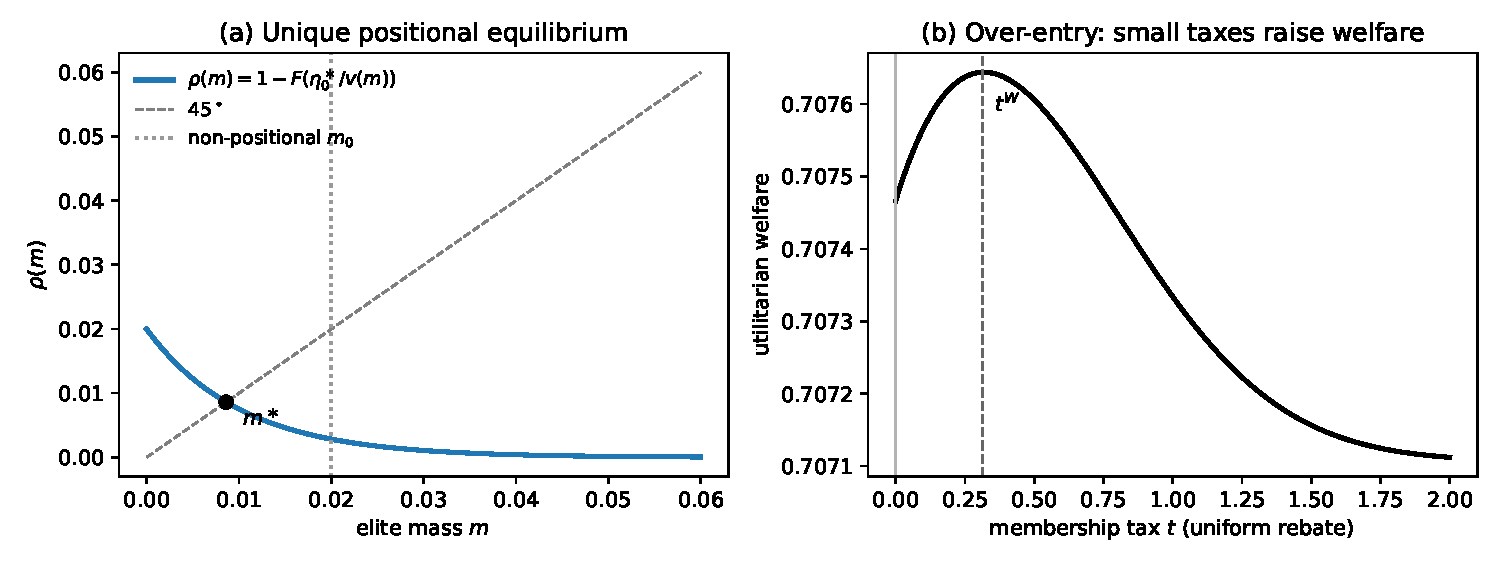
\includegraphics[width=\textwidth]{figures/positional_tax.pdf}
  \caption{The positional equilibrium. Panel (a): the map $\Phi$ of
  \eqref{eq:fixedpoint} is strictly decreasing, giving a unique elite mass
  $M^\ast$, strictly below the non-positional mass $M_0$ (dotted). Panel (b):
  utilitarian welfare as a function of the membership tax $t$ (uniform lump-sum
  rebate); welfare rises for all small taxes --- the signature of over-entry ---
  and peaks at $t^{W}$. Parameters as in Section~\ref{sec:example} with
  $v(M)=1/(1+25M)$.}
  \label{fig:positional}
\end{figure}

\section{Discussion and Planned Extensions}\label{sec:discussion}

\emph{[Working notes; to be developed.]}

\textbf{GDP versus welfare.} Propositions~\ref{prop:coexist}--\ref{prop:decline} and
Theorem~\ref{thm:nocorrection} jointly formalize a distinction the public debate
conflates: what declines as elite status spreads is what statistical agencies
measure, not what agents maximize. Any diagnosis of ``inefficiency'' from output or
TFP data alone presumes status utility does not count --- a normative stance that
should be argued, not assumed.

\textbf{The elite pay puzzle.} In our equilibria elite managers accept \emph{lower}
net incomes --- they pay for status. Observed elite compensation premia are the
opposite. The model points to two reconciliations to be developed: scarcity rents on
the elite characteristic when the supply of status is capped (the positional
extension), and heterogeneity in ability bundled with elite membership. The
membership-price decomposition \eqref{eq:prices} shows exactly where such premia must
enter: as negative prices on a scarce characteristic, as in
\citet[Section~9.3.6]{ellickson2006organization}.

\textbf{Absolute versus positional status as an empirical question.} The paper's
two halves assign opposite policy conclusions to observationally similar worlds ---
wasteful elite institutions persist in both --- so the operative question is which
preference structure obtains. The halves do differ observably:
positional status implies self-damped responses of elite-sector size to demand
shifts (Proposition~\ref{prop:positional}(ii)) and predicts that historical
expansions of elite institutions dilute the premium attached to them, while
absolute status implies proportional pass-through. Developing this into a sharper
empirical strategy is on the agenda for the framing phase.

\textbf{The elite pay puzzle, revisited.} Positional scarcity also supplies the
first of the two reconciliations anticipated above: with $v$ strictly decreasing,
the elite characteristic is in endogenously limited supply, and extensions in which
firms compete for a capped pool of incumbent elites will shift $q_{4.1}$ toward
scarcity rents --- observed premia --- without disturbing the marginal entrant's
status discount.

\textbf{Dynamics (next phase).} The overlapping-generations extension makes $k$ a
state variable: parents value their children's status, finance tuition and bequests,
and the within-period allocation is the equilibrium of
Section~\ref{sec:equilibrium} at the current $k_t$. Because the elite sector burns
resources, the transition map inherits Proposition~\ref{prop:decline}: when status is
a luxury, growth expands the elite sector, which erodes the resource base that
finances it. Multiple steady states and rational-expectations decline paths ---
every generation optimizing, no generation deceived --- are the objects of study.

\appendix

\section{Derivations and Proofs}\label{app:derivations}

All computations in this appendix are verified symbolically in
\texttt{analysis/static\_model.py}.

\subsection{Demand and indirect utility}
An agent with net income $w$ solves $\max_{x_1,x_2} D\sqrt{x_1x_2}$ subject to
$x_1+p_2x_2=w$, giving $x_1=w/2$, $x_2=w/(2p_2)$, and indirect utility
$D\,w/(2\sqrt{p_2})$.

\subsection{Dominated lists}
\begin{lemma}\label{lem:dominated}
At any prices satisfying \eqref{eq:prices} with $r,\tau r>0$, every feasible list
other than the five in Section~\ref{sec:model} is strictly dominated: (i) schooling
with no job yields $D\leq\delta_s<1$ and net income $k-q_j<k$, dominated by leisure;
(ii) schooling plus a laborer job multiplies the laborer's $D$ by $\delta_s<1$ and
subtracts tuition, dominated by the same laborer job alone; (iii) double schooling
adds a factor $\delta_s$ and tuition, dominated by the single required school; (iv)
an elite-school graduate cannot hold membership $m_{3.1}$ nor a serious-school
graduate $m_{4.1}$ (consumption sets), so no other manager lists are feasible.
\qed
\end{lemma}

\subsection{Proof of Lemma~\ref{lem:characterization}}
\emph{Budget balance.} Schools: $q_1-r=0$, $q_2-\tau r=0$ by \eqref{eq:prices}.
Competent firms: $q_{3.1}+2q_{3.2} - c + p_2\phi = (k-r-\mu k) + 2(k-\lambda k) - c +
p_2\phi = 0$ by \eqref{eq:p2}. Elite firms: $q_{4.1}+2q_{4.2} - \beta c +
p_2\alpha\phi = 0$ reduces, using \eqref{eq:p2}, to $w_E = Z$, which is
\eqref{eq:etastar}. \emph{Optimization.} By Lemma~\ref{lem:dominated} only the five
vocational choices need comparison; by construction of \eqref{eq:wages} and
\eqref{eq:cutoff}, types below $\eta^\ast$ are indifferent among the four non-elite
choices and strictly prefer them to the elite path, types above strictly prefer the
elite path, and the marginal type is indifferent. \emph{Consistency and material
balance.} The stated measures fill every group type in the required proportions;
market clearing \eqref{eq:clearing} solves
\begin{equation}\label{eq:nclosed}
  n \;=\; \frac{k - (1-3m^\ast)\frac{k}{2} - m^\ast\left[\frac{w_E}{2} +
  w_{L^\ast} + \tau r + \beta c\right]}
  {\frac{w_M}{2} + w_L - \frac{3k}{2} + r + c},
\end{equation}
positive under Assumption~\ref{ass:interior}. \emph{Walras.} Substituting
\eqref{eq:nclosed} and \eqref{eq:etastar} into the $y_2$ market, demand
$\sum \text{(measures)}\times w/(2p_2)$ equals supply $\phi(n+\alpha m^\ast)$
identically (machine-verified). Uniqueness of the interior configuration follows
because \eqref{eq:wages}--\eqref{eq:etastar} are implied by indifference and budget
balance whenever all memberships are active, and \eqref{eq:nclosed} is linear in
$n$. \qed

\subsection{Proof of Proposition~\ref{prop:coexist}}
Subtracting the two firm budget-balance conditions, $p_2\phi(1-\alpha) =
(w_M - w_E) - 2(w_{L^\ast}-w_L) - (\beta-1)c - (\tau-1)r$ after substituting
\eqref{eq:prices}; the left side is positive iff $\alpha<1$, given $p_2>0$. \qed

\subsection{Proof of Proposition~\ref{prop:decline}}
$\eta^\ast$ solves \eqref{eq:etastar}, which contains no object depending on $F$;
a FOSD shift weakly raises $1-F(\eta)$ pointwise, strictly at $\eta^\ast$ by the
strict-increase assumption on $F$, so $m^\ast$ rises. Differentiating $Y =
\phi(n+\alpha m^\ast)$ with $n$ from \eqref{eq:nclosed},
\[
\frac{dY}{dm^\ast} \;=\; \phi\left(\alpha - 1 + \frac{d(n+m^\ast)}{dm^\ast}\right),
\qquad
\operatorname{sign}\frac{dY}{dm^\ast} = \operatorname{sign}\big[\alpha(c+r) -
(\beta c + \tau r)\big],
\]
where the second equality is by direct computation (machine-verified): the
denominator of \eqref{eq:nclosed} equals $\tfrac12[2c+2r+(\mu+2\lambda\hspace{1pt}{-}\hspace{1pt}3)k]>0$
and the numerator of $\alpha-1+d(n+m^\ast)/dm^\ast$ reduces to
$\alpha(c+r)-(\beta c+\tau r)$ over that denominator. \qed

\section{Verification of Framework Assumptions}\label{app:assumptions}

\emph{Consumption sets.} $X_a = \R^2_+\times\Lists_a$ with $\Lists_a$ the lists
satisfying the schooling prerequisites and the at-most-one-school, at-most-one-job
bounds; the membership bound is $M=2$. Free upward disposal in private goods holds.
The correspondence $a\mapsto X_a$ is constant in $a$ (types differ only through
$u$), hence measurable.

\emph{Utility.} $u(x,\ell;\eta)$ is continuous and strictly increasing in $x$ for
each $\ell$, and jointly measurable since $\eta\mapsto D(\ell;\eta)$ is continuous
and $a\mapsto\eta_a$ measurable.

\emph{Desirable endowments.} $u_a(e_a,0) = h(k,0) = 0$. If
$u_a(x,\ell)>0$ then $x\gg 0$, so any reduction $x'\leq x$, $x'\neq x$, remains in
$X_a$ (consumption sets impose no lower bound above zero); hence endowments are
desirable in the sense of \citet[Section~9.4]{ellickson2006organization}, and their
Theorem~1 delivers membership of every equilibrium state in the strong core and
strong Pareto optimality.

\emph{Existence.} Not invoked: Lemma~\ref{lem:characterization} exhibits equilibrium
in closed form. (For non-interior parameter configurations, existence follows from
Theorem~2 of \citealt{ellickson2006organization} upon verifying group
irreducibility; this is routine but omitted until needed.)

\section{Positional Extension: Proofs}\label{app:positional}

All computations are verified in \texttt{analysis/positional\_model.py}.

\subsection{Proof of Proposition~\ref{prop:positional}}
The occupational-indifference conditions for non-elite choices do not involve $M$,
so \eqref{eq:wages} and \eqref{eq:p2} are unchanged, as is the elite break-even
income $w_E=Z$ from firm budget balance. The cutoff type solves
$(1+\eta v(M))\,\delta_s\delta_m w_E = k$, giving \eqref{eq:positional-cutoff};
sorting is strict above and below the cutoff because
\eqref{eq:positional-utility} is strictly increasing in $\eta$ for fixed $M$.
Consistency of $M$ with sorting is \eqref{eq:fixedpoint}. Since $v$ is continuous
and strictly decreasing and $F$ is continuous and strictly increasing, $\Phi$ is
continuous and strictly decreasing, with $\Phi(0)=1-F(\eta^\ast_0)<1$ and
$\Phi(1)\geq 0$; a unique fixed point $M^\ast\in[0,1)$ exists by the intermediate
value theorem, and $M^\ast>0$ whenever $F$ has unbounded support. (i) Since
$v(M^\ast)<1$ for $M^\ast>0$, $\eta^\ast=\eta^\ast_0/v(M^\ast)>\eta^\ast_0$, so
$M^\ast=1-F(\eta^\ast)<1-F(\eta^\ast_0)=M_0$. (ii) A FOSD shift raises
$1-F(\cdot)$ pointwise, shifting $\Phi$ up; with $\Phi$ strictly decreasing, the
fixed point rises, but the induced fall in $v$ raises the cutoff, damping the
increase: formally $dM^\ast = d\Phi/(1+|\partial\Phi/\partial M|) < d\Phi = dM_0$.
(iii) Immediate, since given $M^\ast$ the remaining conditions coincide with those
of Lemma~\ref{lem:characterization}. \qed

\subsection{Proof of Proposition~\ref{prop:inefficiency}}
Work at the equilibrium of Proposition~\ref{prop:positional}. Shutting one elite
triple and moving its three members to leisure at their reservation utility changes
aggregate excess demand by $(A_e,B_e)$ in (input, output):
\[
A_e = \tau r + \beta c + \tfrac{w_E}{2} + w_{L^\ast} - \tfrac{3k}{2},
\qquad
B_e = -\alpha\phi + \frac{w_E + 2w_{L^\ast} - 3k}{2p_2},
\]
and elite-firm budget balance implies $A_e + p_2 B_e = 0$. Opening one competent
triple staffed from the (indifferent) leisure pool changes excess demand by
$(-A_c, B_c)$ with $A_c = c + r + (w_M+2w_L-3k)/2$, $B_c = \phi -
(w_M+2w_L-3k)/(2p_2)$, and competent budget balance implies $A_c = p_2 B_c$. Both
vectors are orthogonal to $(1,p_2)$, hence collinear; shutting mass $dM>0$ of
elite triples and opening $dn = (A_e/A_c)\,dM$ competent triples restores material
balance in both goods \emph{exactly} (machine-verified). All movers and all
non-elite agents are at reservation utility throughout, so no agent is worse off.
The elite mass falls to $M^\ast-dM$, so $v$ rises, and every inframarginal elite's
utility rises by $\eta\,[v(M^\ast-dM)-v(M^\ast)]\,\delta_s\delta_m w_E
h$-units~$>0$. Finally, transfer an arbitrarily small amount of each good from the
(strictly better off) elites to all agents pro rata: by continuity the elites
remain strictly better off, and strict monotonicity makes almost every agent
strictly better off. The resulting state is feasible and strictly Pareto dominates
the equilibrium state; the grand coalition can implement it, so the state is
blocked and not in the core. \qed

\subsection{Planner cutoff condition, the wedge \eqref{eq:wedge}, and
Proposition~\ref{prop:tax}}
Consider the one-parameter family of feasible states indexed by the cutoff
$\hat\eta$, constructed as in the proof of Proposition~\ref{prop:inefficiency}
(members outside the elite held at reservation utility; material balance restored
via the competent margin). Elite utility is $U(\eta,\hat\eta) =
(1+\eta v(M(\hat\eta)))\,\delta_s\delta_m w_E\, H$ with $M(\hat\eta) =
1-F(\hat\eta)$ and $H \equiv 1/(2\sqrt{p_2})$. Differentiating aggregate elite
utility and using $M'(\hat\eta)=-f(\hat\eta)$:
\[
\frac{d}{d\hat\eta}\int_{\hat\eta}^{\infty}\! U\, dF
= -\underbrace{U(\hat\eta,\hat\eta)f(\hat\eta)}_{\text{marginal type's utility}}
+ \underbrace{f(\hat\eta)\left|v'(M)\right| \delta_s\delta_m w_E H
\int_{\hat\eta}^{\infty}\!\eta\, dF}_{\text{de-dilution of inframarginals}} .
\]
At an interior optimum the marginal type's \emph{surplus} over reservation utility
equals the second term divided by $f(\hat\eta)$; converting to income units by
dividing by the marginal type's marginal utility of income
$(1+\hat\eta v)\delta_s\delta_m H$ gives the wedge \eqref{eq:wedge}. At
laissez-faire the marginal surplus is zero while $\Omega>0$: over-entry.
For Proposition~\ref{prop:tax}: (i) with tax $t$ and rebate $T=tM$, the entrant's
income becomes $w_E = Z - t$ and the fixed-point map remains continuous and
strictly decreasing, so uniqueness persists and $M(t)$ is strictly decreasing for
small $t$ (machine-verified in the example, monotone by the same argument as
Proposition~\ref{prop:positional}); (ii) at $t=0$ every private margin is at a
first-order optimum, so the derivative of utilitarian welfare reduces to the
uninternalized de-dilution term, which is strictly positive; equating the marginal
entrant's income loss to the wedge gives $t^\ast=\Omega$; (iii) $dM/dt<0$ and
condition \eqref{eq:decline} give $dY/dt>0$ by Proposition~\ref{prop:decline}.
The global welfare-maximizing tax in the numerical example, which accounts for all
equilibrium feedback including the rebate, is computed in
\texttt{analysis/positional\_model.py}. \qed

\bibliographystyle{chicago}
\bibliography{elite-status-refs}

\end{document}
